\documentclass[12pt, a4paper]{article}

\usepackage[utf8]{inputenc}
\usepackage[english]{babel}

\usepackage[left=3.00cm, right=3.00cm, top=3.00cm, bottom=3.00cm]{geometry}

\usepackage{parskip}

% Math typesetting packages
\usepackage{amsmath}
\usepackage{amssymb}
\usepackage{amsfonts}

\newcommand{\graphicsfolder}{".."}

\usepackage{tikz}
\usetikzlibrary{calc}
\usetikzlibrary{math}
\usetikzlibrary{matrix}
\usetikzlibrary{shapes.misc}

\begin{document}
    \subsection*{Unsecured}
    \begin{center}
    \scalebox{0.9}{%
        \begin{tikzpicture}
            % !TEX root = ./test-graphics.tex

\tikzmath{
    \arrowyoffset = 7;
    \arrowcenteryoffset = 7;
    \toparrowyoffset = \arrowcenteryoffset + \arrowyoffset;
    \bottomarrowyoffset = \arrowcenteryoffset - \arrowyoffset;
    \arrowtoboxpadding = 5;
}
\coordinate (center) at (0,0);
\node (dealer) at (center) [
    draw,
    fill=white!80!gray,
    very thick,
    minimum width=3cm,
    minimum height=2cm,
    align=center,
    rounded corners=.50cm,
] {Derivatives\\dealer};

\node (counterparty) at ($(dealer.west) + (-5, 0)$) [
    draw,
    very thick,
    minimum width=3cm,
    minimum height=2cm
] {Counterparty};

\node (exchange) at ($(dealer.east) + (5, 0)$) [
    draw,
    dashed,
    very thick,
    minimum width=3cm,
    minimum height=2cm,
] {Exchange};

\node (funding) at ($(dealer.south) + (0, -4)$) [
    draw,
    very thick,
    minimum width=3cm,
    minimum height=2cm,
] {Prime broker};

% Dealer - Counterparty relations
\draw[->, thick] 
    ([yshift=\bottomarrowyoffset pt, xshift=-\arrowtoboxpadding pt]dealer.south west) -- 
    ([yshift=\bottomarrowyoffset pt, xshift= \arrowtoboxpadding pt]counterparty.south east)
    node[near start, fill=white, inner sep=0pt] {
        
\includegraphics[width=0.60cm]{\graphicsfolder/source-of-funding-costs/contract}
    };
\draw[<-, thick] 
    ([yshift=\toparrowyoffset pt, xshift=-\arrowtoboxpadding pt]dealer.south west) -- 
    ([yshift=\toparrowyoffset pt, xshift= \arrowtoboxpadding pt]counterparty.south east)
    node[near end, fill=white, inner sep=2pt] {
        \$\$\$
    };

% Dealer - Exchange relations
\draw[<-, thick] 
    ([yshift=\bottomarrowyoffset, xshift= \arrowtoboxpadding pt]dealer.south east) -- 
    ([yshift=\bottomarrowyoffset, xshift=-\arrowtoboxpadding pt]exchange.south west)
    node[near end, fill=white, inner sep=0pt] {
        
\includegraphics[width=0.60cm]{\graphicsfolder/source-of-funding-costs/contract}
    };
\draw[->, thick] 
    ([yshift=\toparrowyoffset, xshift= \arrowtoboxpadding pt]dealer.south east) -- 
    ([yshift=\toparrowyoffset, xshift=-\arrowtoboxpadding pt]exchange.south west)
    node[near start, fill=white, inner sep=2pt] {
        \$\$\$
    };

\draw[<->, thick, draw=blue] 
    ([yshift=-\bottomarrowyoffset, xshift= \arrowtoboxpadding pt]dealer.north east) -- 
    ([yshift=-\bottomarrowyoffset, xshift=-\arrowtoboxpadding pt]exchange.north west)
    node [pos=0.4, fill=white, inner sep=0pt] {
        
\includegraphics[width=0.65cm]{\graphicsfolder/source-of-funding-costs/collateral}
    };
\draw[<->, thick, draw=red] 
    ([yshift=-\toparrowyoffset, xshift= \arrowtoboxpadding pt]dealer.north east) -- 
    ([yshift=-\toparrowyoffset, xshift=-\arrowtoboxpadding pt]exchange.north west)
    node [pos=0.6, fill=white, inner xsep=2pt, inner ysep=0] {
        OIS
    };

% Dealer - Funding relations
\draw[<->, thick, draw=blue]
    ([xshift=-\arrowyoffset, yshift=-\arrowtoboxpadding]dealer.south) --
    ([xshift=-\arrowyoffset, yshift= \arrowtoboxpadding]funding.north)
    node[midway, fill=white, inner xsep=2pt, inner ysep=0, align=center, rotate=90] {
        Funding
    };
\draw[<->, thick, draw=red]
    ([xshift=\arrowyoffset, yshift=-\arrowtoboxpadding]dealer.south) --
    ([xshift=\arrowyoffset, yshift= \arrowtoboxpadding]funding.north)
    node[midway, fill=white, inner xsep=2pt, inner ysep=0, align=center, rotate=90] {
        OIS + S
    };
        \end{tikzpicture}
    }
    \end{center}

    \subsection*{Secured}
    \begin{center}
    \scalebox{0.9}{%
    \begin{tikzpicture}
        % !TEX root = ./test-graphics.tex

% !TEX root = ./test-graphics.tex

\tikzmath{
    \arrowyoffset = 7;
    \arrowcenteryoffset = 7;
    \toparrowyoffset = \arrowcenteryoffset + \arrowyoffset;
    \bottomarrowyoffset = \arrowcenteryoffset - \arrowyoffset;
    \arrowtoboxpadding = 5;
}
\coordinate (center) at (0,0);
\node (dealer) at (center) [
    draw,
    fill=white!80!gray,
    very thick,
    minimum width=3cm,
    minimum height=2cm,
    align=center,
    rounded corners=.50cm,
] {Derivatives\\dealer};

\node (counterparty) at ($(dealer.west) + (-5, 0)$) [
    draw,
    very thick,
    minimum width=3cm,
    minimum height=2cm
] {Counterparty};

\node (exchange) at ($(dealer.east) + (5, 0)$) [
    draw,
    dashed,
    very thick,
    minimum width=3cm,
    minimum height=2cm,
] {Exchange};

\node (funding) at ($(dealer.south) + (0, -4)$) [
    draw,
    very thick,
    minimum width=3cm,
    minimum height=2cm,
] {Prime broker};

% Dealer - Counterparty relations
\draw[->, thick] 
    ([yshift=\bottomarrowyoffset pt, xshift=-\arrowtoboxpadding pt]dealer.south west) -- 
    ([yshift=\bottomarrowyoffset pt, xshift= \arrowtoboxpadding pt]counterparty.south east)
    node[near start, fill=white, inner sep=0pt] {
        
\includegraphics[width=0.60cm]{\graphicsfolder/source-of-funding-costs/contract}
    };
\draw[<-, thick] 
    ([yshift=\toparrowyoffset pt, xshift=-\arrowtoboxpadding pt]dealer.south west) -- 
    ([yshift=\toparrowyoffset pt, xshift= \arrowtoboxpadding pt]counterparty.south east)
    node[near end, fill=white, inner sep=2pt] {
        \$\$\$
    };

% Dealer - Exchange relations
\draw[<-, thick] 
    ([yshift=\bottomarrowyoffset, xshift= \arrowtoboxpadding pt]dealer.south east) -- 
    ([yshift=\bottomarrowyoffset, xshift=-\arrowtoboxpadding pt]exchange.south west)
    node[near end, fill=white, inner sep=0pt] {
        
\includegraphics[width=0.60cm]{\graphicsfolder/source-of-funding-costs/contract}
    };
\draw[->, thick] 
    ([yshift=\toparrowyoffset, xshift= \arrowtoboxpadding pt]dealer.south east) -- 
    ([yshift=\toparrowyoffset, xshift=-\arrowtoboxpadding pt]exchange.south west)
    node[near start, fill=white, inner sep=2pt] {
        \$\$\$
    };

\draw[<->, thick, draw=blue] 
    ([yshift=-\bottomarrowyoffset, xshift= \arrowtoboxpadding pt]dealer.north east) -- 
    ([yshift=-\bottomarrowyoffset, xshift=-\arrowtoboxpadding pt]exchange.north west)
    node [pos=0.4, fill=white, inner sep=0pt] {
        
\includegraphics[width=0.65cm]{\graphicsfolder/source-of-funding-costs/collateral}
    };
\draw[<->, thick, draw=red] 
    ([yshift=-\toparrowyoffset, xshift= \arrowtoboxpadding pt]dealer.north east) -- 
    ([yshift=-\toparrowyoffset, xshift=-\arrowtoboxpadding pt]exchange.north west)
    node [pos=0.6, fill=white, inner xsep=2pt, inner ysep=0] {
        OIS
    };

% Dealer - Funding relations
\draw[<->, thick, draw=blue]
    ([xshift=-\arrowyoffset, yshift=-\arrowtoboxpadding]dealer.south) --
    ([xshift=-\arrowyoffset, yshift= \arrowtoboxpadding]funding.north)
    node[midway, fill=white, inner xsep=2pt, inner ysep=0, align=center, rotate=90] {
        Funding
    };
\draw[<->, thick, draw=red]
    ([xshift=\arrowyoffset, yshift=-\arrowtoboxpadding]dealer.south) --
    ([xshift=\arrowyoffset, yshift= \arrowtoboxpadding]funding.north)
    node[midway, fill=white, inner xsep=2pt, inner ysep=0, align=center, rotate=90] {
        OIS + S
    };

\draw[<->, thick, draw=fundingcolor] 
    ([yshift=-\bottomarrowyoffset, xshift=-\arrowtoboxpadding pt]dealer.north west) -- 
    ([yshift=-\bottomarrowyoffset, xshift= \arrowtoboxpadding pt]counterparty.north east)
    node (collateral) [pos=0.6, fill=white, inner sep=0pt] {
        
\includegraphics[width=0.40cm]{\graphicsfolder/source-of-funding-costs/collateral}
    };


\draw[<->, thick, draw=ratecolor] 
    ([yshift=-\toparrowyoffset, xshift=-\arrowtoboxpadding pt]dealer.north west) -- 
    ([yshift=-\toparrowyoffset, xshift= \arrowtoboxpadding pt]counterparty.north east)
    node [pos=0.4, fill=white, inner xsep=2pt, inner ysep=0] {
        OIS
    };
    \end{tikzpicture}
    }
    \end{center}

    \subsection*{Secured example}
    \begin{center}
    \scalebox{0.9}{%
    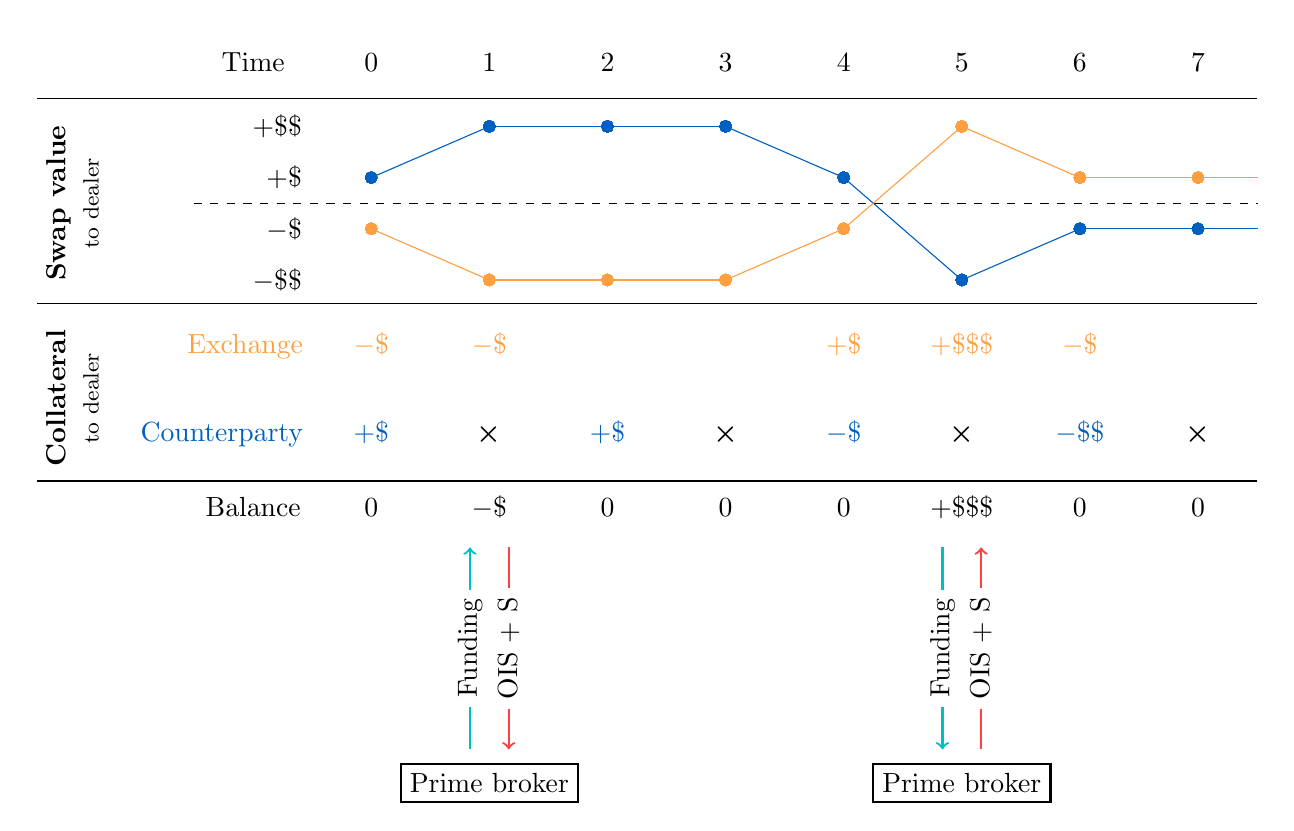
\begin{tikzpicture}
        % !TEX root = ./test-graphics.tex

\colorlet{exchangecolor}{-red!50!yellow!75}
\colorlet{counterpartycolor}{red!50!yellow!75}
\colorlet{fundingcolor}{-red!75}
\colorlet{ratecolor}{red!75}

\matrix [
    matrix of nodes,
    nodes = {
        minimum width = 1.5cm,
        minimum height = 0.65cm
    },
    nodes in empty cells,
    column 1/.append style = {nodes={minimum width=1.2cm}},
    column 2/.append style = {anchor=base east},
    row 6/.append style = {nodes={color=counterpartycolor, minimum height=1cm}},
    row 7/.append style = {nodes={color=exchangecolor, minimum height=1cm}},
] (value) {
    & Time & 0 & 1 & 2 & 3 & 4 & 5 & 6 & 7 \\
    \hline
    & &  &   &   &   &   &   &   &   \\
    & &  &   &   &   &   &   &   &   \\
    & &  &   &   &   &   &   &   &   \\
    & &  &   &   &   &   &   &   &   \\
    \hline
    & Exchange & $-\$$ & $-\$$ &       &   & $+\$$ & $+\$\$\$$ & $-\$$   &   \\
    & Counterparty & $+\$$ &   \textcolor{black}{$\boldsymbol{\times}$}    & $+\$$ & \textcolor{black}{$\boldsymbol{\times}$}  & $-\$$ &   \textcolor{black}{$\boldsymbol{\times}$}  & $-\$\$$ &  \textcolor{black}{$\boldsymbol{\times}$} \\
    \hline
    & Balance & 0     & \node (funding1-in) {$-\$$};      & \node (funding1-out) {0};     
    &       0 & 0     & \node (funding2-out) {$+\$\$\$$}; & \node (funding2-in) {0};  & 0 \\
};

\draw[dashed] ($(value-4-2.west)!0.5!(value-3-2.west)$) -- ($(value-4-10.east)!0.5!(value-3-10.east)$);
% \node () at ([xshift=0.25cm] $(value-4-10.east)!0.5!(value-3-10.east)$) {$0$};

\foreach \labl [count=\row from 2] in {$+\$\$$, $+\$$, $-\$$, $-\$\$$} {
    \node[anchor=east] () at ([xshift=0cm] value-\row-3.west) {\labl};
}
\node [align=center, rotate=90, anchor=north] () at ($(value-4-1.west)!0.5!(value-3-1.west)$) 
    {\textbf{Swap value} \\ \footnotesize to dealer};
\node [align=center, rotate=90, anchor=north] () at ($(value-7-1.west)!0.5!(value-6-1.west)$) 
    {\textbf{Collateral} \\ \footnotesize to dealer};

\foreach \from/\to [count=\col from 3] in {2/1, 1/1, 1/1, 1/2, 2/4, 4/3, 3/3} {
    \tikzmath{%
        \from = \from + 1;
        \to = \to + 1;
        \nextcol = \col + 1;
    };
    \pgfmathtruncatemacro{\from}{\from};
    \pgfmathtruncatemacro{\to}{\to};
    \pgfmathtruncatemacro{\nextcol}{\nextcol};
    \draw[exchangecolor] 
        plot[mark=*] (value-\from-\col.center) -- 
        plot[mark=*] (value-\to-\nextcol.center);
}
\draw[exchangecolor] (value-4-10.center) -- (value-4-10.east);

\foreach \from/\to [count=\col from 3] in {3/4, 4/4, 4/4, 4/3, 3/1, 1/2, 2/2} {
    \tikzmath{%
        \from = \from + 1;
        \to = \to + 1;
        \nextcol = \col + 1;
    };
    \pgfmathtruncatemacro{\from}{\from};
    \pgfmathtruncatemacro{\to}{\to};
    \pgfmathtruncatemacro{\nextcol}{\nextcol};
    \draw[counterpartycolor] 
        plot[mark=*] (value-\from-\col.center) -- 
        plot[mark=*] (value-\to-\nextcol.center);
}
\draw[counterpartycolor] (value-3-10.center) -- (value-3-10.east);

\tikzmath{%
    \fundingyshift=-3.5;
    \arrowxshift=7;
    \arrowtoboxpadding = 5;
}
\node [draw, thick] (funding-institution-1) at ([yshift=\fundingyshift cm] funding1-in) {Prime broker};
\draw [<-, draw=fundingcolor, thick] 
    ([xshift=-\arrowxshift pt, yshift=-\arrowtoboxpadding] funding1-in.south) -- ([xshift=-\arrowxshift pt, yshift=\arrowtoboxpadding] funding-institution-1.north)
    node[rotate=90, midway, fill=white] {Funding};
\draw [->, draw=ratecolor, thick] 
    ([xshift=\arrowxshift pt, yshift=-\arrowtoboxpadding] funding1-in.south) -- ([xshift=\arrowxshift pt, yshift=\arrowtoboxpadding] funding-institution-1.north)
    node[rotate=90, midway, fill=white] {OIS + S};

\node [draw, thick] (funding-institution-2) at ([yshift=\fundingyshift cm] funding2-out) {Prime broker};
\draw [->, draw=fundingcolor, thick] 
    ([xshift=-\arrowxshift pt, yshift=-\arrowtoboxpadding] funding2-out.south) -- ([xshift=-\arrowxshift pt, yshift=\arrowtoboxpadding] funding-institution-2.north)
    node[rotate=90, midway, fill=white] {Funding};
\draw [<-, draw=ratecolor, thick] 
    ([xshift=\arrowxshift pt, yshift=-\arrowtoboxpadding] funding2-out.south) -- ([xshift=\arrowxshift pt, yshift=\arrowtoboxpadding] funding-institution-2.north)
    node[rotate=90, midway, fill=white] {OIS + S};
    \end{tikzpicture}
    }
    \end{center}
\end{document}